\documentclass[11pt,a4paper]{article}
\usepackage[margin=2cm]{geometry}
\usepackage{booktabs,tabularx,array,enumitem,xcolor,hyperref,listings,amsmath}
\usepackage[T1]{fontenc}
\usepackage{lmodern}
\usepackage{tikz}
\usetikzlibrary{automata,positioning,arrows.meta}
\hypersetup{colorlinks=true,linkcolor=blue!50!black,urlcolor=blue!50!black}
\newcolumntype{L}{>{\raggedright\arraybackslash}X}
\setlist{nosep,leftmargin=*}
\setlength{\emergencystretch}{3em}
\lstset{language=C,basicstyle=\ttfamily\footnotesize,breaklines=true,columns=fullflexible,keepspaces=true,
  frame=single,framerule=0.3pt,rulecolor=\color{black!30},xleftmargin=2pt,xrightmargin=2pt,
  commentstyle=\color{green!40!black},keywordstyle=\color{blue!60!black},showstringspaces=false}
\newcommand{\lv}[1]{\texttt{#1}}                 % a Live Expressions variable
\newcommand{\run}[1]{\textbf{How to run.} #1}
\newcommand{\see}[1]{\textbf{What you see.} #1}

\title{Microprocessor-Based Product Design 2026/27\\[2pt]\large Assignment 1: WRONG reference solution (planted errors, to test the checker)}
\author{Yohai Ackerman (TA). \textbf{TA only, never handed to students.}}
\date{Draft of \today}

\begin{document}
\maketitle

\section{The project and how to operate it}

\subsection{What is where}
Everything is in \texttt{assignments/ass1/solution/fullSolution/}:

\smallskip\noindent
\begin{tabularx}{\textwidth}{@{}l L@{}}
\toprule
File & Content \\
\midrule
\texttt{ass1\_sol.tex} & this document \\
\texttt{ass1\_sol/} & the STM32CubeIDE project \\
\texttt{ass1\_sol/ass1\_sol.ioc} & \texttt{ass1.ioc}, unchanged except the project name \\
\texttt{Core/Src/main.c} & generated code; the user code adds \texttt{\_\_io\_putchar} (printf to PuTTY, tutorial~2),
  \texttt{ioBoardInit()}, declares \lv{task} (\texttt{USER CODE BEGIN PV}, as the instructions require), and calls
  the task dispatcher in the main loop (\texttt{USER CODE BEGIN 3}) \\
\texttt{Core/Src/io\_board.c}, \texttt{Core/Inc/io\_board.h} & the students' copy, unchanged \\
\texttt{Core/Inc/ass1.h} & task numbers and shared helpers \\
\texttt{Core/Src/ass1\_tasks.c} & the dispatcher: runs the task chosen in \lv{task} \\
\texttt{Core/Src/ass1\_common.c} & \texttt{printBinary}, \texttt{taskDone}, \texttt{showByteOnLeds},
  \texttt{readButtonsHeld}, the debouncer \\
\texttt{Core/Src/bits.c}, \texttt{Core/Inc/bits.h} & B.1: \texttt{bitSet}, \texttt{bitClear}, \texttt{bitToggle},
  \texttt{bitTest} \\
\texttt{Core/Src/partA.c} \ldots\ \texttt{partE.c} & one file per part \\
\bottomrule
\end{tabularx}

\subsection{Opening, building and starting a debug session}
\begin{enumerate}
  \item In STM32CubeIDE: \emph{File $\to$ Import $\to$ General $\to$ Existing Projects into Workspace}, root directory
        \texttt{fullSolution/ass1\_sol}. Build with the hammer (Debug configuration).
  \item Connect the Nucleo (power jumper on E5V, cart power on) and the IO board. Open PuTTY on the ST-LINK COM port (Device
        Manager shows the number), 115\,200 baud, 8N1.
  \item Start a debug session (\emph{Run $\to$ Debug}, or the launch file \texttt{ass1\_sol Debug.launch}) and press
        \emph{Resume} (F8). PuTTY shows the IO board report of \texttt{ioBoardInit()} (all four chips ``found'') and the
        task menu.
  \item Open \emph{Window $\to$ Show View $\to$ Live Expressions}, and add \lv{task} with \emph{Add new expression}.
        Other variables may be added for debugging; it is not required.
\end{enumerate}

\subsection{Choosing a task}
All parts are in one program. The global variable \lv{task} chooses what runs: click its \emph{Value} cell in Live
Expressions while the program runs, type the number, and press Enter. The running task notices the change, returns,
the LEDs and LD2 are switched off, and the new task starts (PuTTY prints \texttt{=== task N ===}). A task that has an
end (A.1, A.2, A.3, B.1, D.1) prints \texttt{=== task N done ===} and waits. To restart the same task (for example
after changing its settings), write \texttt{0}, then the number again. A number that is not in the table prints
\texttt{no task N} and the menu. This is the protocol the students must follow too (the skeleton in the instructions);
their projects can be tested automatically through it.

\smallskip\noindent
\begin{tabularx}{\textwidth}{@{}c L c L@{}}
\toprule
\lv{task} & Runs & \lv{task} & Runs \\
\midrule
0  & idle (start-up value) & 31 & C.1 buttons held \\
11 & A.1 wrap-around & 32 & C.2 level-based counting \\
12 & A.2 hex values, signed and unsigned & 33 & C.3 edge-based counting \\
13 & A.3 integer division & 34 & C.4 debounced counting \\
21 & B.1 bit functions on LD2 & 35 & C.5 debounced counter with \texttt{HAL\_Delay(150)} \\
22 & B.2 one LED walks & 36 & C.5 edge counter with \texttt{HAL\_Delay(150)} \\
23 & B.3 a pair of LEDs walks & 41 & D.1 200 toggles, timed \\
   &  & 42 & D.2 LD2 at a rate from \lv{blinkMs} \\
   &  & 43 & D.3 with \texttt{HAL\_Delay} \\
   &  & 44 & D.3 with \texttt{HAL\_GetTick} \\
   &  & 51 & E armed state, IR sensor, brightening \\
\bottomrule
\end{tabularx}

\smallskip\noindent
Every result line starts with its tag (\texttt{A1:}, \texttt{B2:}, \ldots) in the format the instructions prescribe;
the ``What you see'' blocks below show these lines.

\smallskip\noindent
When watching variables for debugging: Live Expressions shows a value in decimal by default; for the bit patterns of Parts A and B, right-click the
expression and choose another number format (hex or binary), where the view offers it. An \texttt{enum} variable
(\lv{eState}) is shown by name.

\subsection{Status of this solution}
\textbf{Run on the cart (2026-11-04)} by the automatic test, in its shortened form: A.1 and A.2 are caught (A.1 starts at 120, no binary in A.1 and A.2), and every other automatic item is ``works good'', as intended. Parts C and E are the same code as the good solution, which was run with presses and a hand on 2026-11-04; the IR sensor is read through \texttt{IR\_OBSTACLE\_LEVEL} (\texttt{ass1.h}), as there.

The code builds with the CubeIDE toolchain (GCC 14.3, Debug configuration) with 0 warnings (2026-10-28). Parts A,
B and D were run on the board by the automatic test (2026-10-29), and every line and number below matched: D.1 total
101\,201\,ms, D.2 half periods 502 to 503\,ms (\lv{blinkMs} = 500) and 102\,ms (100), D.3 17\,740 and 17\,742\,ms
with \texttt{HAL\_Delay}, 10\,000 and 7\,693\,ms with \texttt{HAL\_GetTick}. With no input, C.1, C.2 and E were run
too: their start lines are as below, and C.2 makes 9\,679 loop passes per second. Presses (C) and the IR sensor (E): see the
good solution's report, where they were run on 2026-11-04.

\subsection{The automatic test}
The skill \texttt{/skl\_prj\_checkAss} runs \texttt{assignments/autotest/assignments\_autotest.py}. It builds a
group's project (with its \texttt{Debug} makefile, or CubeIDE headless if there is none), flashes it, runs A.1 to A.3,
B.1 to B.3 and D.1 to D.3 by writing \lv{task} (and \lv{blinkMs}) over SWD while the program runs, reads the tagged
lines from the COM port, and writes one short comment per task into the sheet ``Assignment 1'' of
\texttt{assignments/autotest/assignments gradings.xlsx}: ``works good'', or what is wrong. Then Claude reads the
group's report against this document and adds ``report: \ldots'' comments where needed. C and E are graded from the
videos. The TA types the points (e.g.\ $-2$); the Total column is 100 plus all of them. One group takes about
3\,minutes on the board, most of it D.1. Close PuTTY and stop any CubeIDE debug session first: both hold the board.

\section{Shared helpers}
\begin{lstlisting}
void printBinary(uint32_t value, uint8_t nBits)   // provided in the instructions (A.1)
{
    printf("0b");
    for (int8_t i = (int8_t)(nBits - 1); i >= 0; i--)
    {
        putchar(((value >> i) & 1u) ? '1' : '0');      // 0b11110000
    }
}

void taskDone(uint8_t myTask)                     // the end of a task that has an end
{
    if (task == myTask)                           // not when stopped early by a new choice
    {
        printf("=== task %u done ===\r\n", myTask);
    }
    while (task == myTask) { }
}

void showByteOnLeds(uint8_t pattern)              // LED n white while bit n is 1
{
    for (uint8_t n = 0; n < N_LEDS; n++)
    {
        uint8_t v = bitTest(pattern, n) ? LED_LEVEL : 0;
        setRGB_led(n, v, v, v);
    }
}

uint8_t readButtonsHeld(void)                     // bit n = 1 while button n is held
{
    return (uint8_t)(~readButtonsRaw()) & 0x0Fu;
}
\end{lstlisting}
\texttt{printBinary} is given to the students in A.1; they call it from their own line-printing
functions. One LED update by \texttt{showByteOnLeds} (B.2, B.3) is 24 I2C writes, about 2\,ms at 400\,kHz; one button read is about
103\,$\mu$s (measured through C.2: 9\,679 loop passes per second).

\section{Part A: variable types, signed and unsigned, wrap-around}

\subsection*{A.1}
\run{Write \lv{task} = 11. The three variables start at 120
and grow by one every 500\,ms; after the start line and 12 steps the task is done.
Measured on the board, the lines come 510\,ms apart: \texttt{HAL\_Delay(500)} waits 501 ticks, and printing the
line takes about 4\,ms more.}

\see{13 lines. Selected ones: the start, steps 6 to 9 (i8 wraps at step 8) and step 12:}
\begin{lstlisting}[language={},basicstyle=\ttfamily\scriptsize]
A1: u8=120 0x78 i8=120 0x78 u16=120 0x0078
A1: u8=126 0x7E i8=126 0x7E u16=126 0x007E
A1: u8=127 0x7F i8=127 0x7F u16=127 0x007F
A1: u8=128 0x80 i8=-128 0x80 u16=128 0x0080
A1: u8=129 0x81 i8=-127 0x81 u16=129 0x0081
A1: u8=132 0x84 i8=-124 0x84 u16=132 0x0084
=== task 11 done ===
\end{lstlisting}

\textbf{Answer.} An $n$-bit variable holds $2^n$ bit patterns. Adding 1 to the largest pattern (all ones) gives a
carry out of the top bit, which has no place to go and is lost, so the result is all zeros:
\begin{itemize}
  \item \texttt{uint8\_t}: $255 + 1 \to 0$; \texttt{uint16\_t}: $65\,535 + 1 \to 0$. Unsigned arithmetic in C is
        defined modulo $2^n$.
  \item \texttt{int8\_t}: $127 + 1 \to -128$. The pattern goes from \texttt{0111\_1111} to \texttt{1000\_0000}; in two's
        complement the top bit has the weight $-128$, so the same pattern now reads as $-128$. (In C the
        \texttt{int8\_t} is first promoted to \texttt{int}, $127 + 1 = 128$ is computed, and converting 128 back into an
        \texttt{int8\_t} wraps it; GCC defines this conversion as modulo $2^8$.)
\end{itemize}
The hex output shows it directly: the same 8 bits, read as unsigned or signed.

\subsection*{A.2}
\run{Write \lv{task} = 12. The six lines are printed once.}

\see{}
\begin{lstlisting}[language={},basicstyle=\ttfamily\scriptsize]
A2: hex=0x7F uint8_t dec=127 raw=0x7F
A2: hex=0x7F int8_t dec=127 raw=0x7F
A2: hex=0xF0 uint8_t dec=240 raw=0xF0
A2: hex=0xF0 int8_t dec=-16 raw=0xFFFFFFF0
A2: hex=0xFFF6 uint16_t dec=65526 raw=0xFFF6
A2: hex=0xFFF6 int16_t dec=-10 raw=0xFFFFFFF6
=== task 12 done ===
\end{lstlisting}

\textbf{Answer.} A hex digit is 4 bits, and the value is $\sum d_k\,16^k$: \texttt{0xF0} $= 15 \cdot 16 + 0 = 240$,
\texttt{0xFFF6} $= 65\,526$. For an unsigned type that is the value. For a signed type of $n$ bits, if the top bit is
1 (the first hex digit is 8 or more), the value is negative: subtract $2^n$. So \texttt{0xF0} as \texttt{int8\_t} is
$240 - 256 = -16$, \texttt{0xFFF6} as \texttt{int16\_t} is $65\,526 - 65\,536 = -10$, and \texttt{0x7F} (top bit 0)
is 127 in both types.

\emph{A negative value printed in hex:} \texttt{printf("\%X", x)} with \texttt{x = -16} prints \texttt{FFFFFFF0}, not
\texttt{F0}. A variable narrower than \texttt{int} is promoted to a 32-bit \texttt{int} when it is passed to
\texttt{printf}; a negative value is sign-extended (the top bit is copied into the 24 new bits), and \texttt{\%X}
prints all 32 bits. Casting to the unsigned type of the same width, \texttt{(uint8\_t)x}, prints \texttt{F0}.

\emph{Note:} \texttt{int8\_t x = 0xF0;} makes GCC warn (``overflow in conversion from int to int8\_t changes value
from 240 to $-16$''): the constant 240 does not fit. The solution writes \texttt{(int8\_t)0xF0} to say it is meant.

\subsection*{A.3}
\run{Write \lv{task} = 13. To try other grades, change \lv{a3Grade1},
\lv{a3Grade2}, then write \lv{task} = 0 and 13.}

\see{\texttt{A3: wrong=77 right=77.5}}
\begin{lstlisting}
a3AvgWrong = (a3Grade1 + a3Grade2) / 2;      // 155 / 2 = 77   (integer division)
a3AvgRight = (a3Grade1 + a3Grade2) / 2.0f;   // 155 / 2.0 = 77.5
\end{lstlisting}
\textbf{Answer.} When both operands of \texttt{/} are integers, C does an integer division, and the fraction is
dropped: 77 instead of 77.5. If either operand is a floating-point value (\texttt{2.0f}, or a cast
\texttt{(float)(a + b) / 2}), the other is converted and the division is done in floating point. Storing the
integer result in a \texttt{float} afterwards (\texttt{float avg = (a + b) / 2;}) does not help: the fraction is
already lost. The sum itself is safe: two \texttt{uint8\_t} are promoted to \texttt{int} before the addition, so
$97 + 58 = 155$ is computed in 32 bits (storing it in a \texttt{uint8\_t} would wrap only above 255).

\emph{Printing a float:} with the default newlib-nano library, \texttt{printf("\%f")} prints nothing until
\emph{Project Properties $\to$ C/C++ Build $\to$ Settings $\to$ MCU Settings $\to$ ``Use float with printf from
newlib-nano''} is ticked. The solution avoids it and prints the tenths by hand.

\section{Part B: bit operations and shifting}

\subsection*{B.1}
\begin{lstlisting}
uint32_t bitSet(uint32_t value, uint8_t bit)    { return value |  (1UL << bit); }
uint32_t bitClear(uint32_t value, uint8_t bit)  { return value & ~(1UL << bit); }
uint32_t bitToggle(uint32_t value, uint8_t bit) { return value ^  (1UL << bit); }
uint8_t  bitTest(uint32_t value, uint8_t bit)   { return (uint8_t)((value >> bit) & 1UL); }
\end{lstlisting}
\run{Write \lv{task} = 21. The sequence runs once: LD2 off; after 1\,s on (set); after 1\,s off (clear); after 1\,s on
(toggle). After each step the bit is read back with \texttt{bitTest(GPIOA->ODR, 5)} and printed. The last result, 1,
lights LED~0 of the IO board (white), and \lv{b1Result} = 1. To see it again, write \lv{task} = 0 and 21.}

\see{\texttt{B1: start LD2=0}, \texttt{B1: set LD2=1}, \texttt{B1: clear LD2=0}, \texttt{B1: toggle LD2=1},
\texttt{B1: LED0=1}, \texttt{=== task 21 done ===}.}

\textbf{Answer.} OR with a mask sets the bit, AND with the inverted mask clears it, XOR flips it, and shifting the bit
down to bit~0 and masking with 1 tests it. The mask is \texttt{1UL << bit}: \texttt{1UL} is 32 bits wide and unsigned,
so even bit~31 of a register is safe. \texttt{GPIOA->ODR = bitSet(GPIOA->ODR, 5)} reads the output register, changes
bit~5 only, and writes it back, so the other pins of port~A keep their levels.

\subsection*{B.2 and B.3}
\begin{lstlisting}
if (b2Pattern == 0x01)      b2Pattern = 0x02;    // the next pattern, chosen by an if chain
else if (b2Pattern == 0x02) b2Pattern = 0x04;
...
else if (b2Pattern == 0x80) b2Pattern = 0x01;    // B.2: back to LED 0
else if (b2Pattern == 0xC0) b2Pattern = 0x81;    // B.3: LEDs 7 and 0
else if (b2Pattern == 0x81) b2Pattern = 0x03;
\end{lstlisting}
\run{Write \lv{task} = 22 (B.2, starts from \texttt{0x01}) or 23 (B.3, starts from \texttt{0x03}). One step per
second, forever, until \lv{task} changes. Measured: 1\,003\,ms per step on average (the LED update, about 2\,ms, and
the line, about 1.3\,ms, come on top of \texttt{HAL\_Delay(1000)}).}

\see{B.2: \texttt{B2: 0b00000001}, \texttt{B2: 0b00000010}, \ldots, \texttt{B2: 0b10000000}, \texttt{B2: 0b00000001},
\ldots\ B.3: \texttt{B3: 0b00000011}, \texttt{B3: 0b00000110}, \ldots, \texttt{B3: 0b11000000}, \texttt{B3: 0b10000001}
(LEDs 7 and 0), \texttt{B3: 0b00000011}, \ldots}

\textbf{Answer (past bit 7).} After \texttt{0x80} the if chain gives \texttt{0x01} again (B.2), and after
\texttt{0xC0} it gives \texttt{0x81}, then \texttt{0x03} (B.3), so the pattern goes on past bit~7. The LEDs are
lit by \texttt{showByteOnLeds}, which tests each bit.

\section{Part C: input triggering}

\subsection*{C.1 Buttons held}
\run{Write \lv{task} = 31. Hold any combination of the four buttons.}

\see{At the start (measured on the board): \texttt{C1: raw=0b00001111 held=0b00000000 count=0}. With button~0
held: \texttt{C1: raw=0b00001110 held=0b00000001 count=1}. With buttons 0 and 2: \texttt{held=0b00000101 count=2}. A
line is printed only when the count changes. On this board bits 4 to 7 of the raw byte read 0.}

\textbf{Answer.} The buttons are active-low, so \texttt{\textasciitilde raw} makes a held button a 1. Bits 4 to 7 of
the PCA9538A carry no button; they read 0, so after the inversion they are 1, and \texttt{\& 0x0F} clears them.
Without the mask the count would include them (4 extra), which is exactly why the instructions ask for it. The count is
the sum of \texttt{bitTest(held, n)} for $n = 0$ to 3.

\subsection*{C.2 to C.5: counting presses}
\run{Write \lv{task} = 32, 33, 34, 35 or 36 for C.2, C.3, C.4, C.5 (debounced) and C.5 (edge). The count runs in
rounds: press button~0 20 times, then button~1. Button~1 prints the result line, \texttt{C3: count=21} (C.2 also gives
the passes per second, \texttt{C2: count=4317 passes=9680}), sets the count back to 0 and starts the next round, so the
3 rounds need no restart. Nothing else is printed while counting, and the LEDs are not used. \lv{cDebounceMs} = 20 and
\lv{cDelayMs} = 150 can be changed while it runs. The hint in the instructions for each version: C.2 much more than
20, C.3 20 or a little more, C.4 exactly 20, C.5 much less than 20.}

\begin{lstlisting}
// button 1: once per press (released -> pressed); then ignored for 0.5 s, so its bounces print nothing
static uint8_t roundEnded(RoundButton *b, uint8_t held, uint32_t tick)
{
    uint8_t now = bitTest(held, 1);
    uint8_t pressed = now && !b->before;
    b->before = now;
    if (pressed && (tick - b->lastEnd >= ROUND_IGNORE_MS)) { b->lastEnd = tick; return 1; }
    return 0;
}
\end{lstlisting}
One loop pass reads all four buttons in one I2C read, so button~1 costs the loop nothing extra. Without the LED
update after each count, a pass is only that read (about 103\,$\mu$s): the same conditions as the TA measurements with
\texttt{bounceCheck400}, on which the expected numbers below rest.

\subsection*{C.2 Level-based}
\begin{lstlisting}
held = readButtonsHeld();
if (bitTest(held, 0)) cCount++;          // every pass while button 0 is held
loops++;                                 // passes per second = loops / round time
\end{lstlisting}
\textbf{Expected.} About 9\,700 loop passes per second (measured 9\,679, with no press): one pass is one I2C read of
the button chip, about 103\,$\mu$s. A press of about 150\,ms adds about $0.15 \times 9\,700 \approx 1\,450$, so 20
presses give a count of tens of thousands, different every round. \textbf{Answer:} the level-based counter counts loop
passes while the button is held, not presses; the count is (passes per second) $\times$ (total time held).

\subsection*{C.3 Edge-based}
\begin{lstlisting}
uint8_t now     = readButtonsHeld();
uint8_t pressed = now & (uint8_t)~before;   // 1 where a button went from released to pressed
before = now;
if (bitTest(pressed, 0)) cCount++;
\end{lstlisting}
\textbf{Expected} (TA measurement): natural presses 20 to 23 per 20.
\textbf{Answer:} a mechanical contact bounces: while it closes or opens, it makes and breaks contact several times
within about a millisecond. A read that falls in such a gap sees ``released'', the next one ``pressed'', and the edge
counter counts an extra press. The bounce pulses are shorter than one read (about 0.1\,ms), so only some are caught,
and the count is sometimes 20, sometimes more.

\subsection*{C.4 Debounced}
\begin{lstlisting}
uint8_t debounceUpdate(Debouncer *d, uint8_t sample, uint32_t tick, uint32_t stableMs)
{
    if (sample != d->raw) { d->raw = sample; d->changeTick = tick; }      // moved: restart
    else if ((sample != d->stable) && (tick - d->changeTick >= stableMs))
    {
        d->stable = sample;                 // stable for 20 ms: accept
        return sample;                      // 1 only for an accepted press
    }
    return 0;
}
\end{lstlisting}
\textbf{Expected:} 20 of 20 in every round. A bounce gap restarts the 20\,ms timer, so the new state is accepted only
once the contact has settled.

\subsection*{C.5 Missing presses}
\textbf{Expected} (TA measurement, quick taps of 110 to 130\,ms, \texttt{HAL\_Delay(150)}): debounced (35) 0 of 20,
edge (36) about 11 of 20. Button~1 has to be held a little longer here, at least one loop period of 151\,ms, or the
round does not end.

\textbf{Answer.} With the delay, the button is read once per loop pass, about 151\,ms (\texttt{HAL\_Delay(150)} waits
at least 150\,ms and up to 151, plus 0.1\,ms for the read). A tap shorter than that is seen by at most one read, or by
none if it falls between two reads. The edge version needs one read inside the tap, so it catches a tap with a
probability of about (tap duration) / (loop period), and loses the rest. The debounced version needs the pressed state
to be seen again at least 20\,ms later; the next read comes 151\,ms later, when a quick tap is already over, so the
change is never confirmed and it loses all of them. In general, a reliable reading needs a loop period much shorter
than the shortest input event: here the ``other task'' of 150\,ms makes that impossible, and the cure is to keep the
loop short (non-blocking code, Part~D) or to let the input interrupt the program (EXTI, Assignment~2).

\smallskip\noindent
\begin{tabularx}{\textwidth}{@{}l c c c L@{}}
\toprule
Version & Round 1 & Round 2 & Round 3 & Expected \\
\midrule
C.2 level & & & & tens of thousands, different each round \\
C.3 edge & & & & 20 to 23 \\
C.4 debounced & & & & 20 \\
C.5 debounced + delay & & & & 0 \\
C.5 edge + delay & & & & about 11 \\
\bottomrule
\end{tabularx}

\section{Part D: LED blinking and timing}
\run{Part D is one program with the rest. D.1: write \lv{task} = 41; it
stops by itself after 200 toggles, and prints the total as \texttt{D1: toggles=200 total=<ms>}. D.2: write \lv{task} = 42, then change
\lv{blinkMs} (default 500) while LD2 blinks; each toggle prints \texttt{D2: t=<tick> LD2=<0 or 1>}. D.3: write \lv{task} = 43 (\texttt{HAL\_Delay}) or 44
(\texttt{HAL\_GetTick}); the time of every 10 blinks of each LED is printed as \texttt{D3: led=0 ms=<n>} (or \texttt{led=1}). The rates are \lv{d3FreqMilliHz0} = 1000 and \lv{d3FreqMilliHz1} = 1300 (in mHz).}

\subsection*{D.1}
\begin{lstlisting}
for (d1Toggles = 0; d1Toggles < 200; )
{
    HAL_GPIO_TogglePin(LD2_GPIO_Port, LD2_Pin);
    d1Toggles++;
    printf("D1: toggle=%lu of 200, elapsed t=%6lu ms, LD2=%u, status OK\r\n", ...);  // about 60 characters
    HAL_Delay(500);
}
d1TotalMs = HAL_GetTick() - start;
\end{lstlisting}
\textbf{Expected:} $200 \times 500\,\text{ms} = 100\,000$\,ms by calculation; measured 101\,201\,ms (predicted below: 101\,200).

\textbf{Answer.} Two things add to the 500\,ms:
\begin{itemize}
  \item The UART. \texttt{printf} sends the line through \texttt{HAL\_UART\_Transmit}, which waits until each character
        has left. One character is 10 bits (start, 8 data, stop): $10 / 115\,200 = 86.8\,\mu$s. A 60-character line
        takes $60 \times 86.8\,\mu\text{s} = 5.2$\,ms, during which the program does nothing else.
  \item \texttt{HAL\_Delay} adds one tick to guarantee the minimum wait (the line \texttt{wait += uwTickFreq}
        in \texttt{stm32g4xx\_hal.c}), so \texttt{HAL\_Delay(500)} waits until 501 ticks have passed.
\end{itemize}
Together, each pass ends 501 ticks after the tick in which the print ended, which is 5 ticks after the pass began:
$5 + 501 = 506$\,ms per pass, and $200 \times 506 = 101\,200$\,ms, 1.2\% more than calculated.

\subsection*{D.2}
\begin{lstlisting}
while (task == TASK_D2)
{
    HAL_GPIO_TogglePin(LD2_GPIO_Port, LD2_Pin);
    printf("D2: t=%lu LD2=%u\r\n", HAL_GetTick(), ...);
    HAL_Delay(blinkMs);                     // read again before every toggle
}
\end{lstlisting}
Each half period lasts between $d + 2$ and $d + 3$\,ms for \lv{blinkMs} $= d$: one extra tick from
\texttt{HAL\_Delay}, and about 1.7\,ms for the \texttt{D2:} line (about 20 characters on the UART). So 500 gives
about 0.995\,Hz, 100 about 4.9\,Hz, 50 about 9.5\,Hz; the \texttt{t=} values show it directly. A new value takes effect at the next
toggle.

\subsection*{D.3}
Theory: one blink is one on and one off, so 10 blinks take 10 periods: LED~0 (1\,Hz) $10 \times 1\,\text{s} =
10\,000$\,ms, LED~1 (1.3\,Hz) $10 / 1.3 = 7\,692$\,ms. Each half period: 500\,ms and 384.6\,ms. The time is measured
from the toggle that starts blink~1 to the toggle that starts blink~11.

\paragraph{With \texttt{HAL\_Delay} (task 43).}
\begin{lstlisting}
blinkerToggle(&led0, &d3Led0Ms);   HAL_Delay(500);
blinkerToggle(&led1, &d3Led1Ms);   HAL_Delay(385);
\end{lstlisting}
\textbf{Expected:} about 17\,740\,ms for \emph{both} LEDs. Each pass toggles each LED once and waits for both delays,
$501 + 386 = 887$\,ms (the toggles themselves, 3 I2C writes each, about 0.25\,ms, fall inside the same ticks); 10
blinks are 20 passes. \textbf{Answer:} with blocking delays the two LEDs cannot have their own rates: the program
waits for one LED while the other one is due, so both LEDs blink at the rate set by the sum of the delays, 0.56\,Hz
instead of 1 and 1.3\,Hz.

\paragraph{Report question: can the two rates be produced exactly with \texttt{HAL\_Delay} alone?}
\textbf{Answer: approximately yes, exactly no.} The half periods are 500\,ms and $5000/13 = 384.615$\,ms, in the ratio
13\,:\,10. A common base step that fits both a whole number of times is $500/13 = 38.46$\,ms: a loop with one short
delay per pass and two counters toggles LED~0 every 13 passes and LED~1 every 10 passes.
\begin{lstlisting}
HAL_Delay(37);                                   // one pass: about 38 ms (HAL_Delay adds one tick)
if (++count0 == 13) { count0 = 0; toggle LED 0; }
if (++count1 == 10) { count1 = 0; toggle LED 1; }
\end{lstlisting}
The ratio of the two rates is then exactly 1.3, but both are off by the error of the base step:
\begin{itemize}
  \item 38.46\,ms is not a whole number of ticks. A pass of 38\,ms gives 9\,880 and 7\,600\,ms for 10 blinks (1.012 and
        1.316\,Hz); a pass of 39\,ms (\texttt{HAL\_Delay(38)}) gives 10\,140 and 7\,800\,ms (0.986 and 1.282\,Hz), about
        1.2\% either way. Alternating 38 and 39\,ms passes (7 of 38 and 6 of 39 make 500) brings the average right.
  \item Each \texttt{HAL\_Delay(n)} waits from $n$ to $n + 1$ ticks, depending on where in the tick it is called, and the
        work in the pass (3 I2C writes per toggle, about 0.25\,ms) adds to it. A program that only waits never reads a
        clock, so it cannot see these errors, and they add up from pass to pass without limit.
\end{itemize}
Exact long-term rates need a clock: \texttt{HAL\_GetTick} deadlines advanced by the period (task 44) keep every toggle
within one tick of its ideal time, forever. Accept any answer that finds the common step (or a merged timeline of the
46 toggles in 10\,s) and explains why it is still not exact: whole-ms steps, the extra tick, the time of the work.

\paragraph{With \texttt{HAL\_GetTick} (task 44).}
\begin{lstlisting}
uint32_t nowUs = HAL_GetTick() * 1000u;
if ((int32_t)(nowUs - next0) >= 0) { blinkerToggle(&led0, &d3Led0Ms); next0 += 500000; }
if ((int32_t)(nowUs - next1) >= 0) { blinkerToggle(&led1, &d3Led1Ms); next1 += 384615; }
\end{lstlisting}
\textbf{Expected:} LED~0 10\,000\,ms, LED~1 7\,692 or 7\,693\,ms, each within about 2\,ms of the theory: one tick,
plus the \texttt{D3:} line that the other LED may be printing (about 20 characters, 1.7\,ms on the UART) when a
toggle is due. The deadlines are not moved by that delay, so it does not add up.
\textbf{Answer:} each LED has its own deadline, and the loop never waits, so each LED toggles within one tick of its
deadline, whatever the other does. Three details decide the accuracy, and are the differences students are expected
to find:
\begin{itemize}
  \item Advance the deadline by the period (\texttt{next += half}), not to ``now'' (\texttt{last = now}). With
        \texttt{last = now}, every toggle starts its wait from the moment it was noticed, up to 1\,ms late plus the
        I2C write, and the errors add up over 20 toggles.
  \item The half period of 1.3\,Hz is 384.615\,ms, not a whole number of ticks. A deadline in whole ms (385) gives
        $20 \times 385 = 7\,700$\,ms, 8\,ms (0.1\%) too long. Keeping the deadlines in microseconds lets the toggles
        fall on 384 or 385\,ms, so that the average is right.
  \item The tick is 1\,ms, so a single toggle can be up to 1\,ms off; that does not add up when the deadline is
        advanced by the period.
\end{itemize}
The subtraction \texttt{nowUs - next} is converted to a signed number, so the comparison stays right when the counter
wraps (Part~A again).

\smallskip\noindent
\begin{tabularx}{\textwidth}{@{}l c c L@{}}
\toprule
 & LED 0, 1\,Hz & LED 1, 1.3\,Hz & Why \\
\midrule
Theory & 10\,000\,ms & 7\,692\,ms & 10 periods \\
\texttt{HAL\_Delay} & about 17\,740\,ms & about 17\,740\,ms & both delays in every pass \\
\texttt{HAL\_GetTick}, ms deadlines & 10\,000\,ms & 7\,700\,ms & 385 instead of 384.6\,ms \\
\texttt{HAL\_GetTick}, $\mu$s deadlines (this solution) & 10\,000\,ms & 7\,692\,ms & within about 2\,ms \\
\bottomrule
\end{tabularx}

\section{Part E: integration and logic}
\run{Write \lv{task} = 51. Button~0
arms and disarms (LD2 is on while armed), also during a brightening. PuTTY shows \texttt{E: armed=<0|1>
obstacle=<0|1> v=<value>} whenever \emph{armed} or the obstacle changes, and when a brightening reaches 255, just
before the LEDs switch off (\texttt{v} is the value given to \texttt{setRGB}, after \texttt{gamma2}). Hold a hand in
front of the IR sensor for an obstacle. \lv{eStepMs} = 40 and \lv{eStepSize} = 5 give 51 steps of 40\,ms, about 2\,s
from off to full; \lv{eUseGamma} = 1 makes the steps look even to the eye (\texttt{gamma2} of \texttt{io\_board.h}),
0 gives linear values.}

\paragraph{Truth table of the trigger condition.}
\begin{center}
\begin{tabular}{c c c}
\toprule
armed & obstacle & condition \\
\midrule
0 & 0 & 0 \\
0 & 1 & 0 \\
1 & 0 & 0 \\
1 & 1 & 1 \\
\bottomrule
\end{tabular}
\end{center}

\paragraph{State diagram.}
\begin{center}
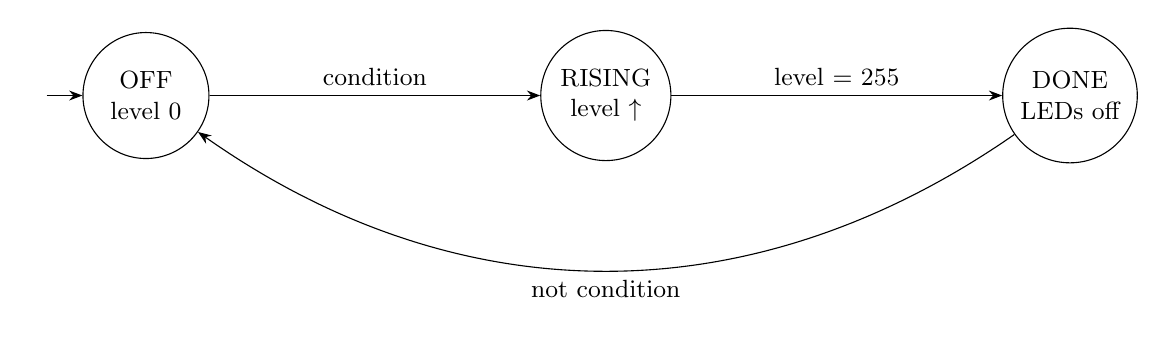
\begin{tikzpicture}[>=Stealth,node distance=2.2cm and 4.2cm,every state/.style={minimum size=1.6cm,align=center,font=\small},
  every edge/.style={draw,->},font=\small]
  \node[state,initial,initial text={}] (off) {OFF\\level 0};
  \node[state,right=of off] (rise) {RISING\\level $\uparrow$};
  \node[state,right=of rise] (done) {DONE\\LEDs off};
  \path (off)  edge node[above] {condition} (rise)
        (rise) edge node[above] {level = 255} (done)
        (done) edge[bend left=35] node[below] {not condition} (off);
\end{tikzpicture}
\end{center}
In RISING the level grows by \lv{eStepSize} every \lv{eStepMs}, whatever the condition does; when 255 has been shown
for one step, the LEDs switch off (DONE). DONE waits until the condition is false, and only then goes back to OFF, where
the next true condition starts a new brightening. So the condition must become false and then true again after a
brightening has ended. If it went false and back to true during the brightening, it is still true in DONE, and nothing
more happens.

\paragraph{The main loop.} The button (debounced, as in C.4) and the IR sensor are read on every pass; the brightness
steps are paced by \texttt{HAL\_GetTick}. Nothing waits, so a press or an obstacle change is never missed (compare C.5),
also during a brightening: \emph{armed} still toggles, and its line is printed, but the brightening goes on.

\paragraph{Test sequence} (also the content of the video \texttt{V\_E}):
\begin{enumerate}
  \item Disarmed, obstacle: nothing happens (condition 0).
  \item Arm (LD2 on), no obstacle: nothing happens.
  \item Armed, hold the obstacle: the LEDs brighten for about 2\,s, then switch off (DONE). Keep the hand there: no
        second brightening.
  \item Remove the hand (OFF) and bring it back: a new brightening.
  \item Remove the hand, or disarm, halfway through a brightening: it still runs to its end.
\end{enumerate}

\section{Grading notes}
\begin{itemize}
  \item Automatic test: A, B.1 to B.3 and D are checked from the PuTTY lines, so a wrong line format or a missing
        \texttt{task} protocol makes the test fail. C.1 to C.5 and E are graded from the videos \texttt{V\_C} and
        \texttt{V\_E}. The test does not see the RGB LEDs of B.2, B.3 and D.3: check in the code that they are lit
        from the variable's bits.
  \item A.1: \texttt{printBinary} is provided; they must call it from a line-printing function of their own (a
        line built by hand bit by bit, or a different binary function, is fine too). The start values and the 12 steps are fixed. A.2: the explanation of \texttt{FFFFFFF0} (promotion and sign extension) is the key point.
  \item B.2 and B.3: patterns chosen with \texttt{if}/\texttt{switch}, a counter mapped to LEDs, or a table, are not
        accepted (the rule in the assignment). The rotation line, or an equivalent \texttt{if (p \& 0x80)} that then uses
        only bit operations, is.
  \item C: no LEDs in C.2 to C.5. Button~1 ends a round and prints once (its bounces must not print a second line);
        nothing is printed while counting. The video shows one round of 20 per version; the report table holds the
        3 rounds of C.2 to C.5. The explanation must use the press duration and the loop time.
  \item D.1: both the UART time (5.2\,ms per line) and the extra tick of \texttt{HAL\_Delay} explain the difference; the
        UART is the larger one.
  \item D.3: the blocking version must show that both LEDs end up at the same rate; the non-blocking version must be
        within a few ms of the theory, and the report must explain any remaining difference.
  \item E: no dimming. A brightening always runs to its end; the next one needs the condition to become false and
        then true after that end. The inputs must be read on every pass, also during a brightening (no
        \texttt{HAL\_Delay} in the stepping); the truth table and a state diagram with the condition on its
        transitions are required.
\end{itemize}

\end{document}
